\subsubsection{pr01}
\label{subsubsec:pr01}
The obtained results were the following:
{
\renewcommand{\arraystretch}{2}
\begin{longtable}[h]{| c | c | c | c | c |}
    \hline
    \textbf{Failures} & \multicolumn{3}{c}{Time limit} & \\
    \hline
    \textbf{Search strategy} & \textbf{\textit{30 sec}} & \textbf{\textit{1 min}} & \textbf{\textit{2 min}} & \textbf{\textit{5 min}} \\
    \hline
    \endhead
    default search                                         & 179.012 & 365.127 &  839.451 & 2.327.625 \\
    \hline
    domWdeg, random                                        & 238.294 & 429.711 &  891.466 & 2.492.341 \\
    \hline
    domWdeg, random, Luby restart L=250                    & 184.952 & 370.280 & 2.617.320 & 2.235.785 \\
    \hline
    \textit{domWdeg, random, Luby restart L=250, LNS 85\%} & 149.239 & 288.638 &  636.876 & 1.925.601 \\
    \hline
    domWdeg, random, Luby restart L=250, LNS 15\%          & 114.333 & 268.527 &  663.974 & 2.088.613 \\
    \hline
    first fail, min                                        & 268.034 & 539.621 &  975.927 & 2.501.499 \\
    \hline
\end{longtable}
}
\begin{figure}[H]
    \centering
    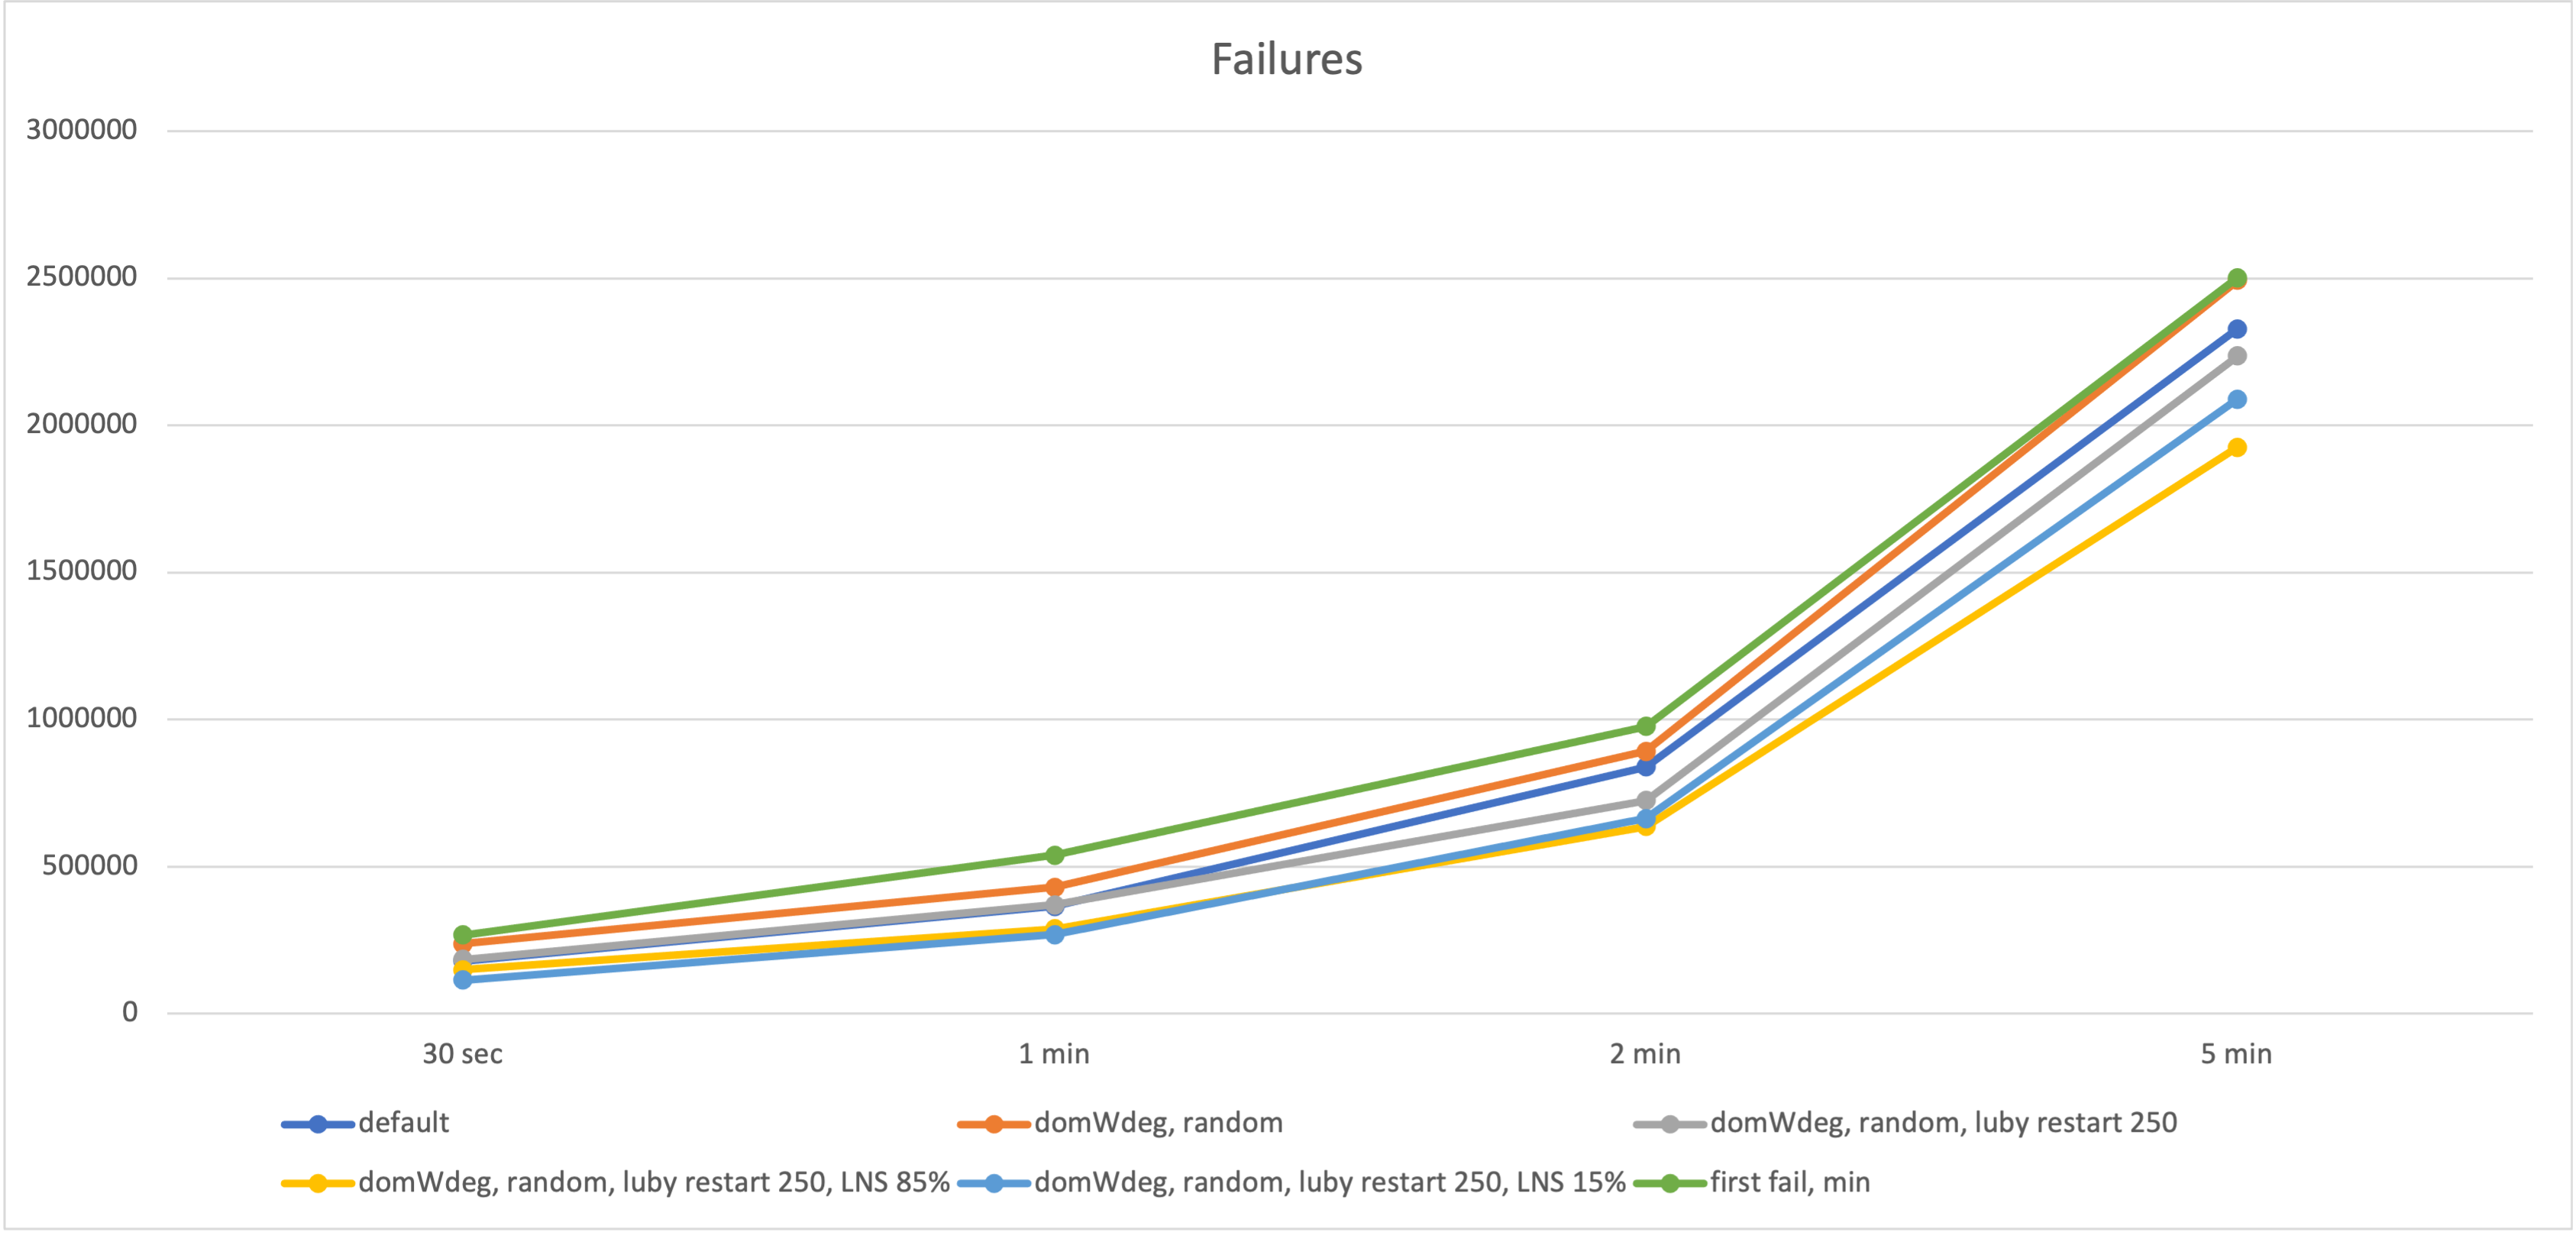
\includegraphics[width=0.8\columnwidth]{../graphs/pr01-failures.png}
    \caption{Failures graph for \textbf{pr01}.}
\end{figure}

{
\renewcommand{\arraystretch}{2}
\begin{longtable}[h]{| c | c | c | c | c |}
    \hline
    \textbf{Objective function} & \multicolumn{3}{c}{Time limit} & \\
    \hline
    \textbf{Search strategy} & \textbf{\textit{30 sec}} & \textbf{\textit{1 min}} & \textbf{\textit{2 min}} & \textbf{\textit{5 min}} \\
    \hline
    \endhead
    default search                                         & 27.140.270 & 26.951.510 & 26.935.140 & 26.612.860 \\
    \hline
    domWdeg, random                                        & 29.242.460 & 29.065.910 & 28.899.840 & 28.788.480 \\
    \hline
    domWdeg, random, Luby restart L=250                    & 26.173.200 & 26.173.200 & 26.173.200 & 26.173.200 \\
    \hline
    \textit{domWdeg, random, Luby restart L=250, LNS 85\%} & 10.973.010 & 10.782.920 & 10.466.080 & 10.466.080 \\
    \hline
    domWdeg, random, Luby restart L=250, LNS 15\%          & 25.982.320 & 25.068.200 & 24.818.310 & 24.550.800 \\
    \hline
    first fail, min                                        & 27.953.160 & 27.953.160 & 27.953.160 & 27.953.160 \\
    \hline
\end{longtable}
}
\begin{figure}[H]
    \centering
    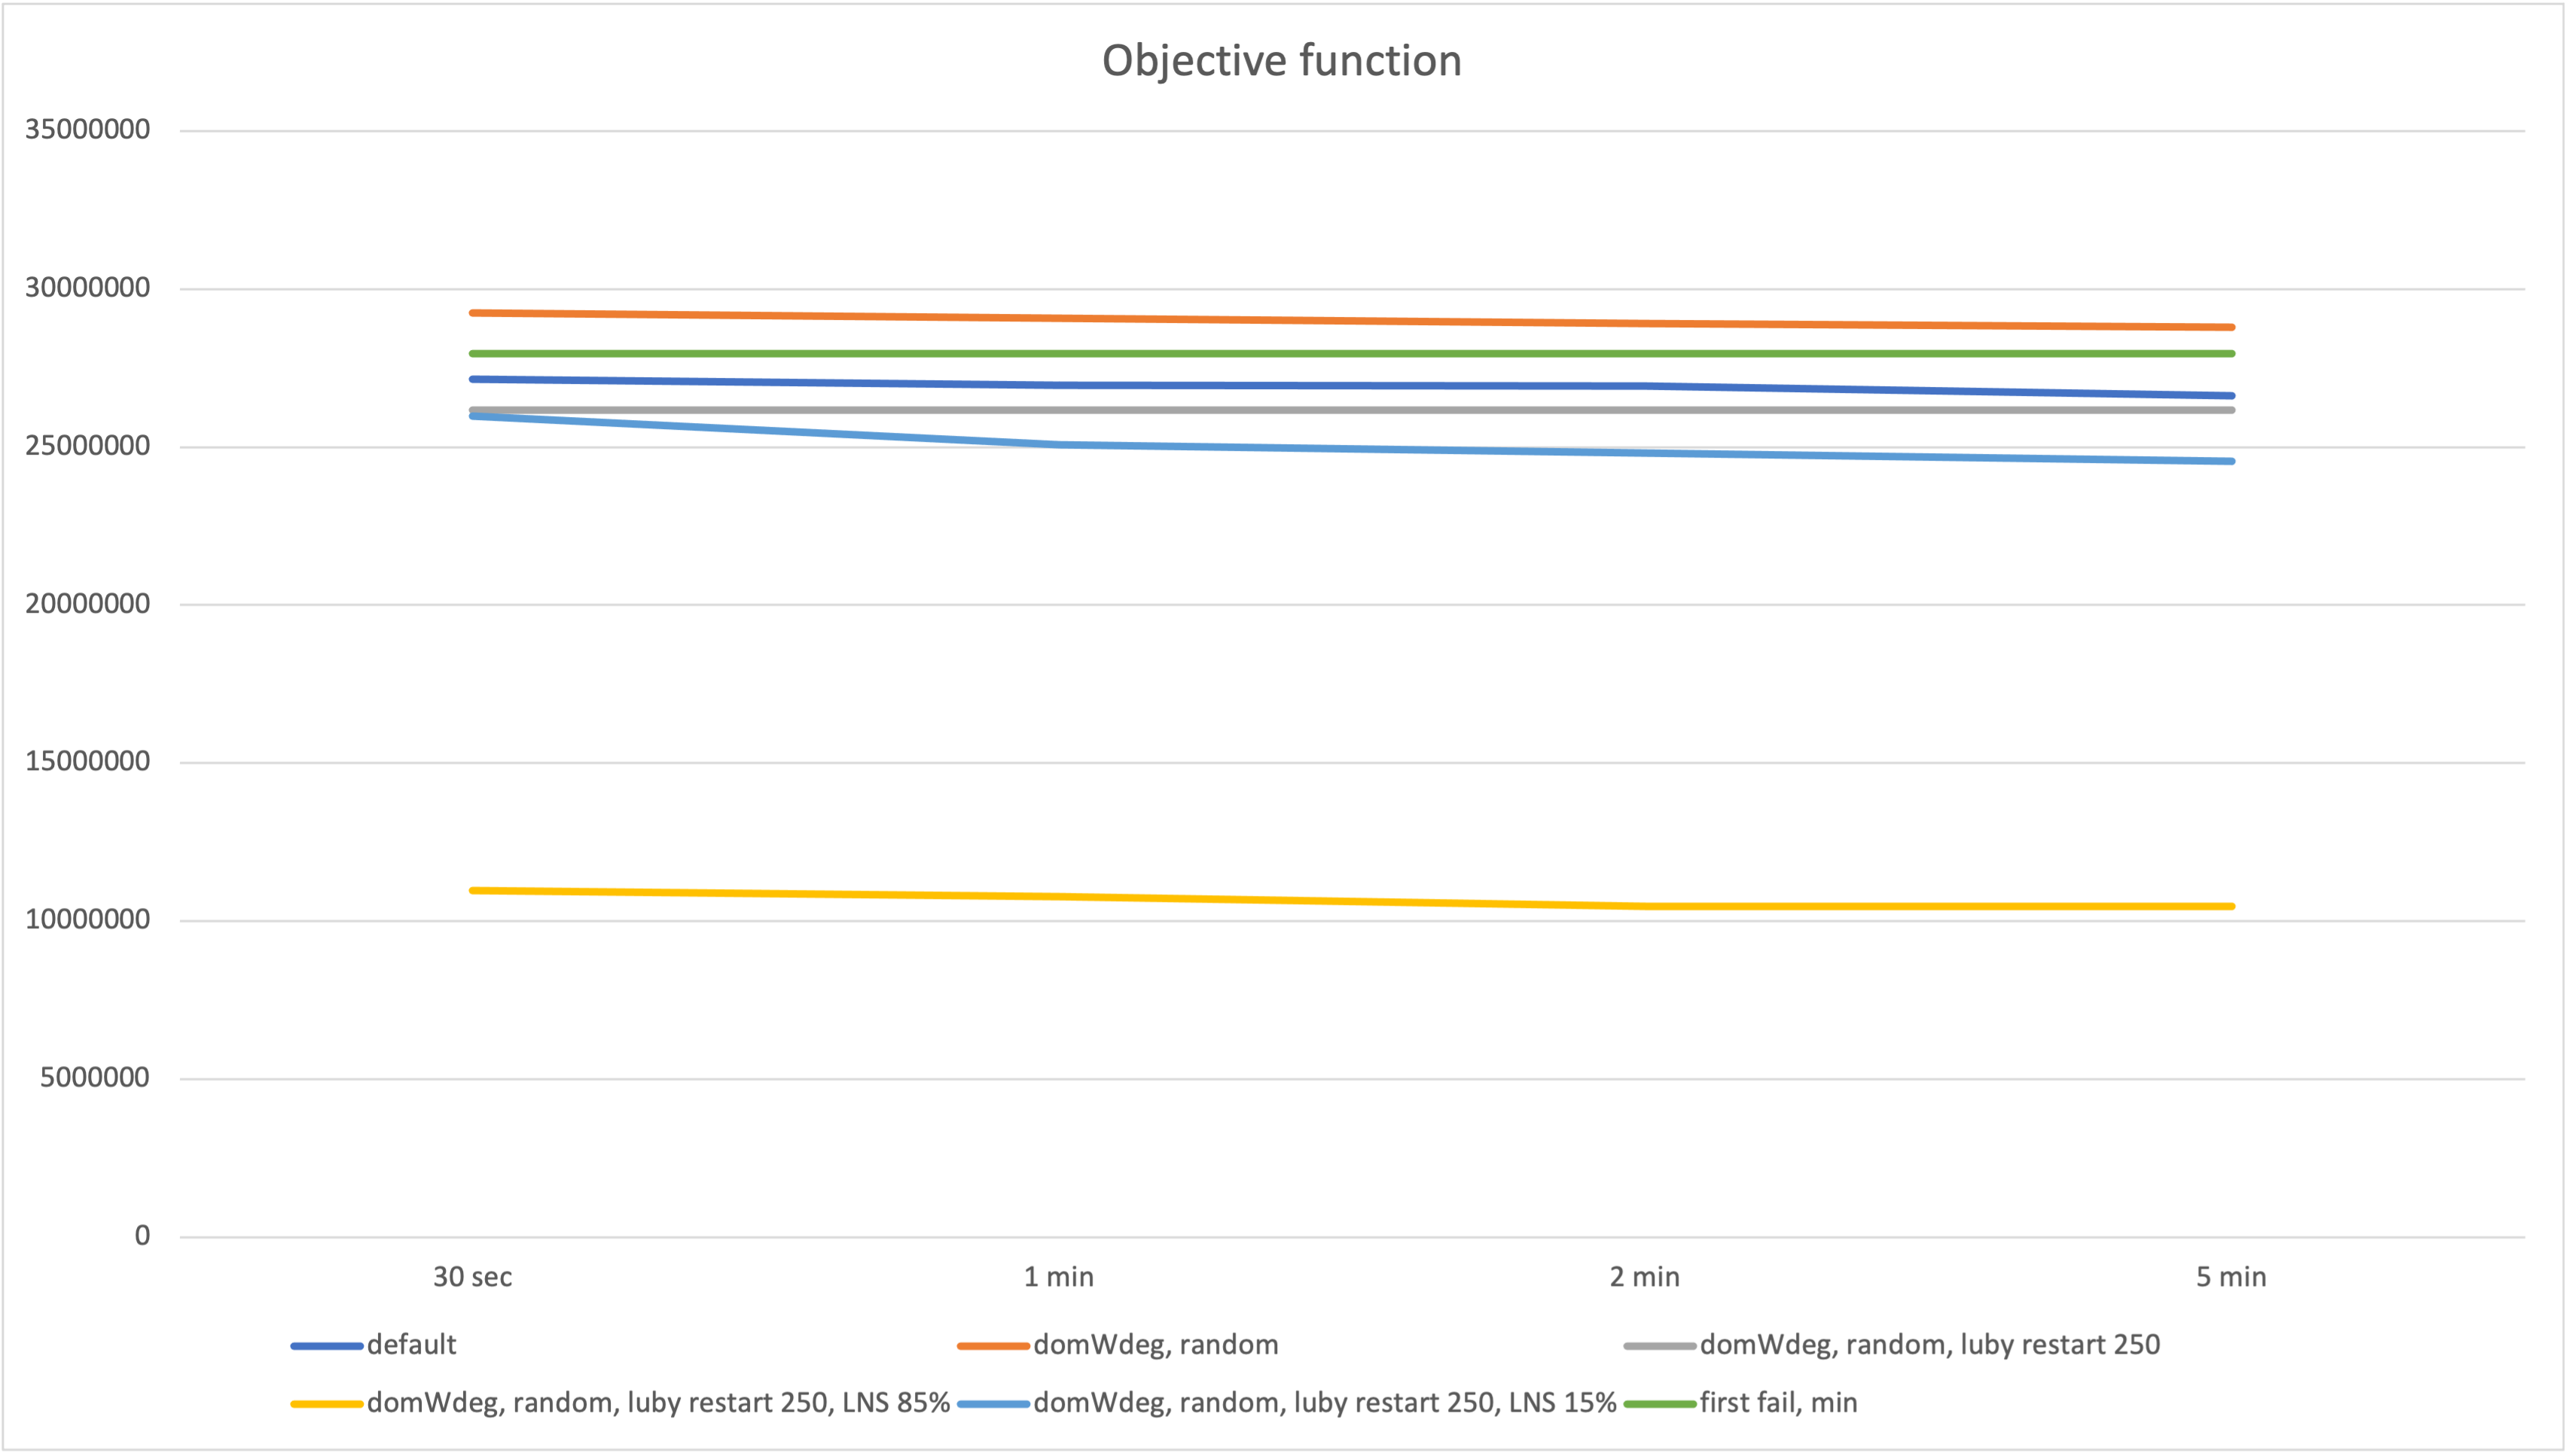
\includegraphics[width=0.8\columnwidth]{../graphs/pr01-objf.png}
    \caption{Objective functions graph for \textbf{pr01}.}
\end{figure}

{
\renewcommand{\arraystretch}{2}
\begin{longtable}[h]{| c | c | c | c |}
    \hline
    \textbf{Weights} & \textbf{Objective function} & \textbf{Total distance} & \textbf{Used vehicles} \\
    \hline
    \endhead
    $\alpha = 10, \beta = 0$ & 10.115.720 & 1.011.572 & 4 \\
    \hline
    $\alpha = 7, \beta = 3$  &  7.064.853 & 1.009.263 & 4 \\
    \hline
    $\alpha = 5, \beta = 5$  &  5.046.335 & 1.009.263 & 4 \\
    \hline
    $\alpha = 3, \beta = 7$  &  2.864.569 &   954.847 & 4 \\
    \hline
    $\alpha = 0, \beta = 10$ &         40 & 3.210.707 & 4 \\
    \hline
\end{longtable}
}
\begin{figure}[H]
    \centering
    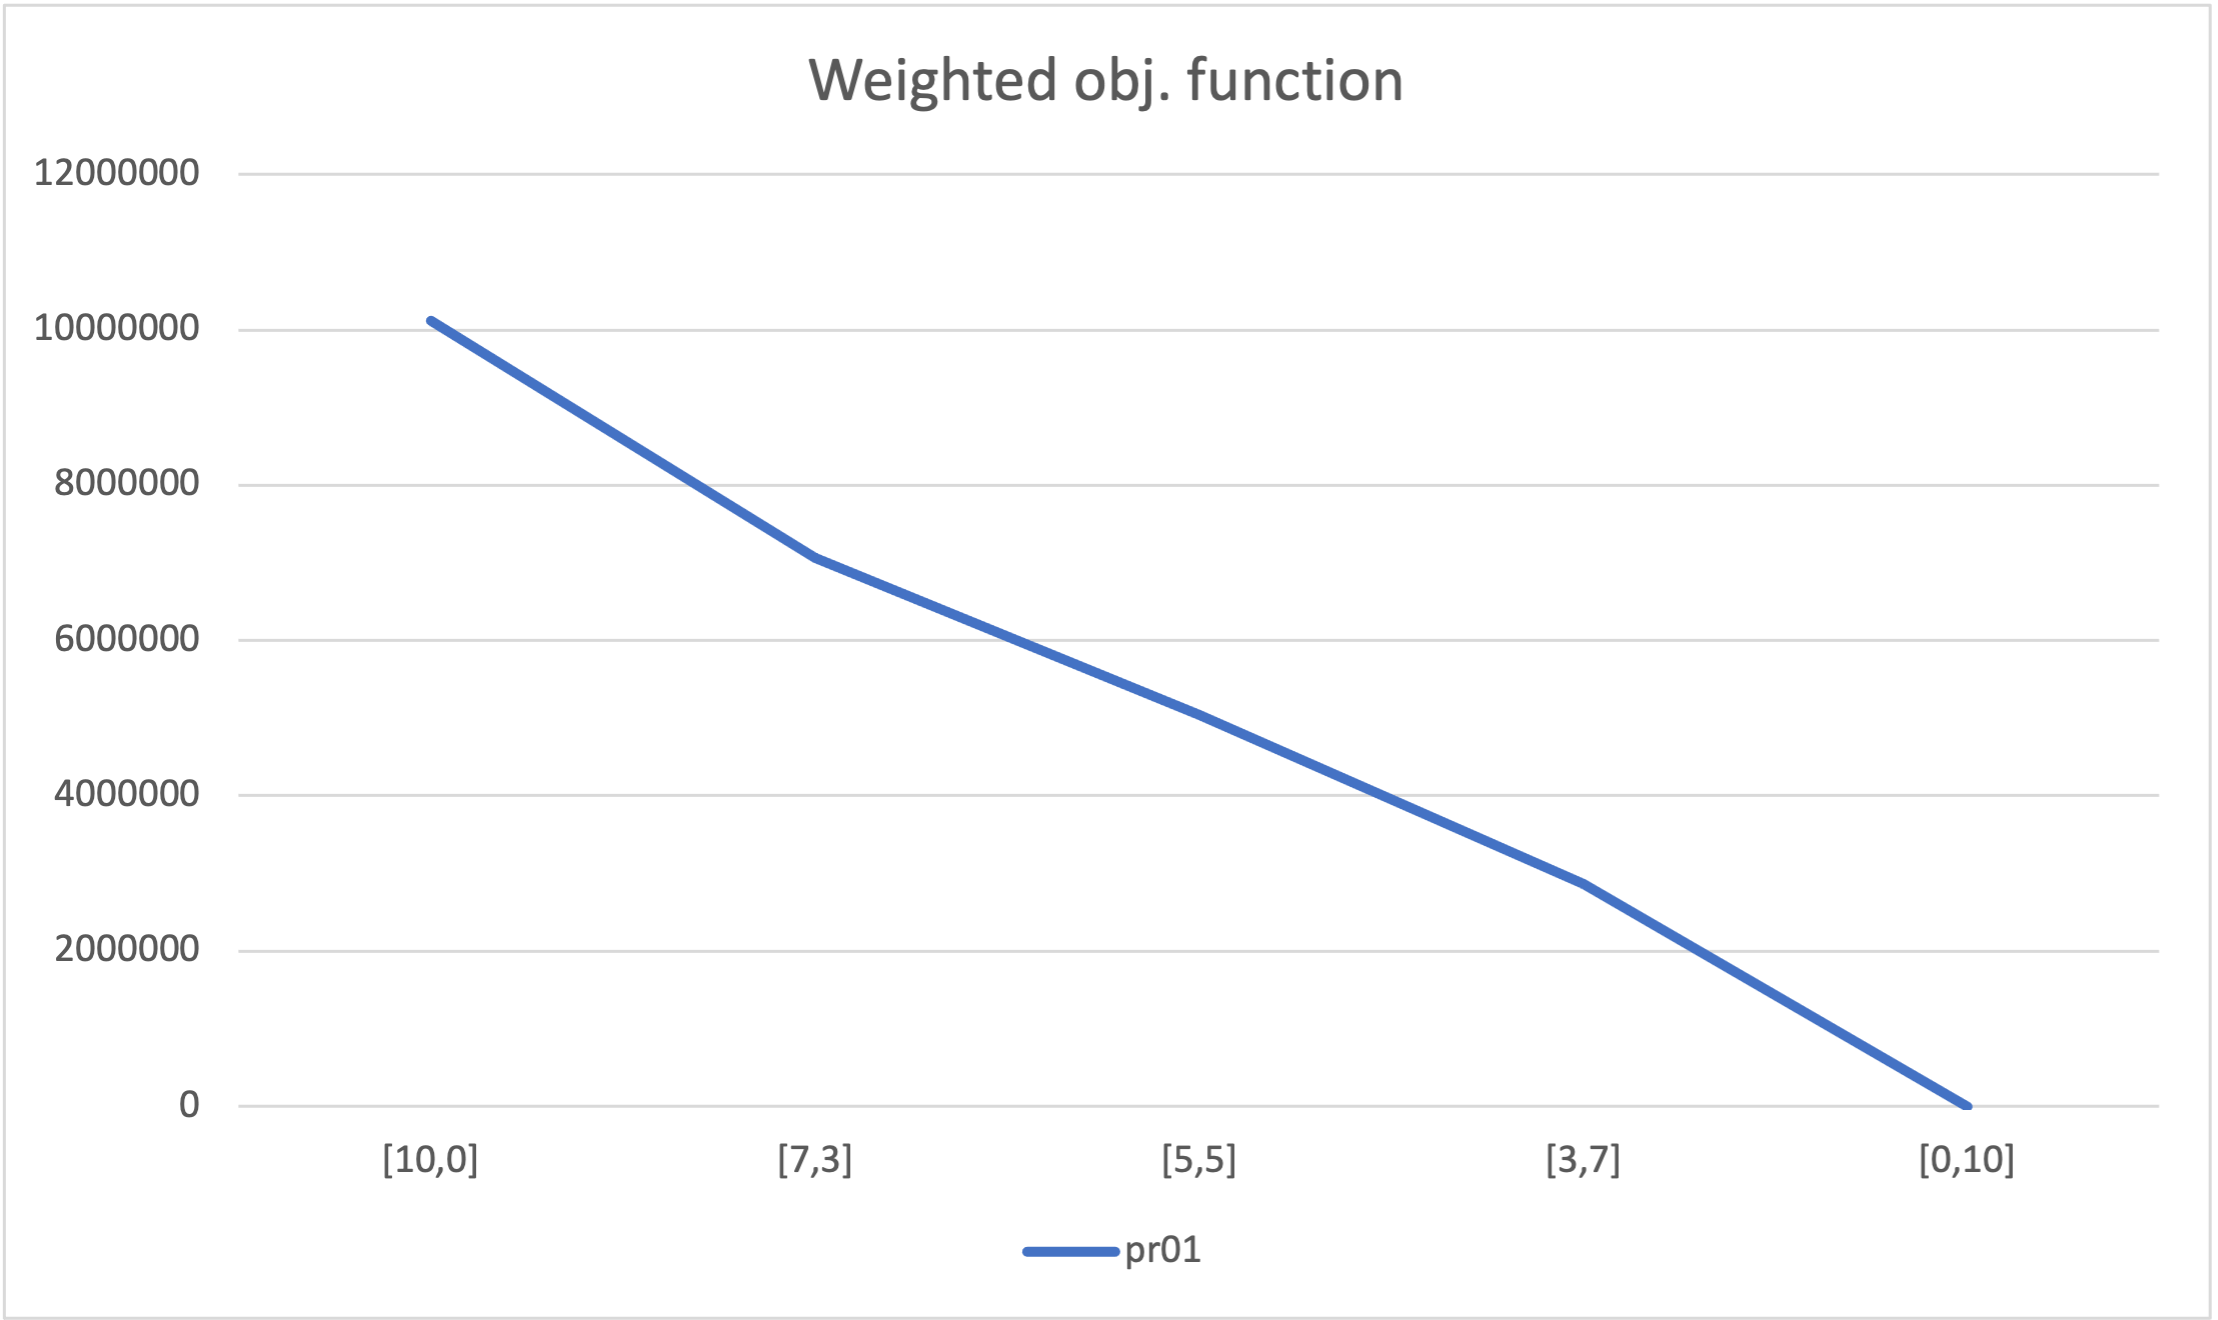
\includegraphics[height=0.25\textheight]{../graphs/pr01-wobjf.png}
    \caption{Weighted objective functions graph for \textbf{pr01}.}
\end{figure}

\begin{figure}[H]
    \centering
    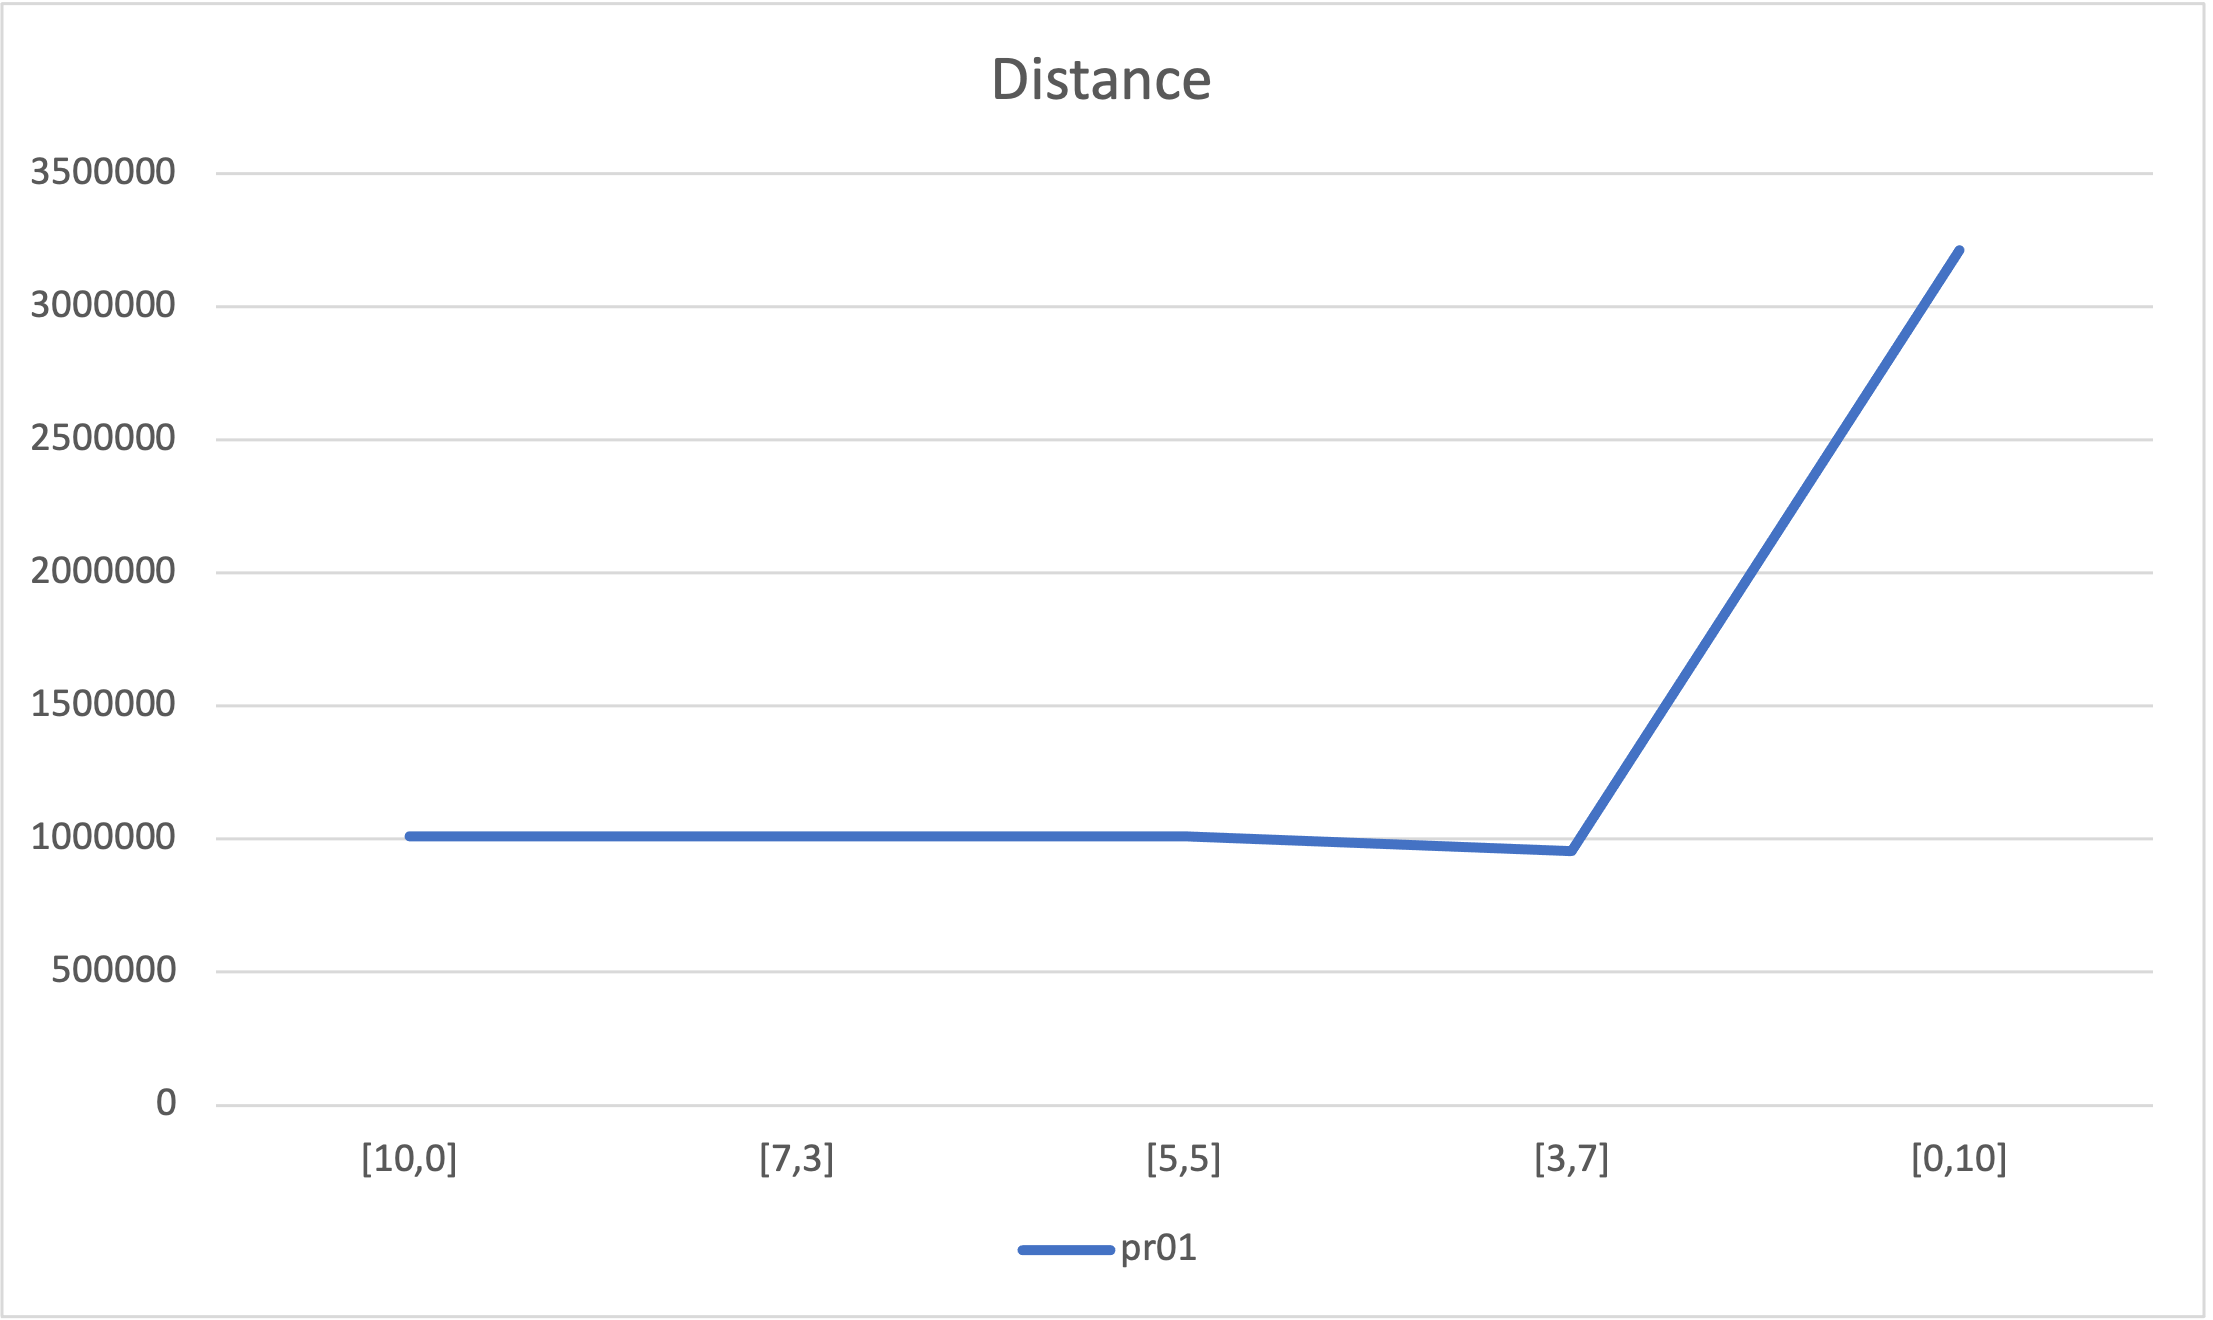
\includegraphics[height=0.25\textheight]{../graphs/pr01-distance.png}
    \caption{Distances graph for \textbf{pr01}.}
\end{figure}

\begin{figure}[H]
    \centering
    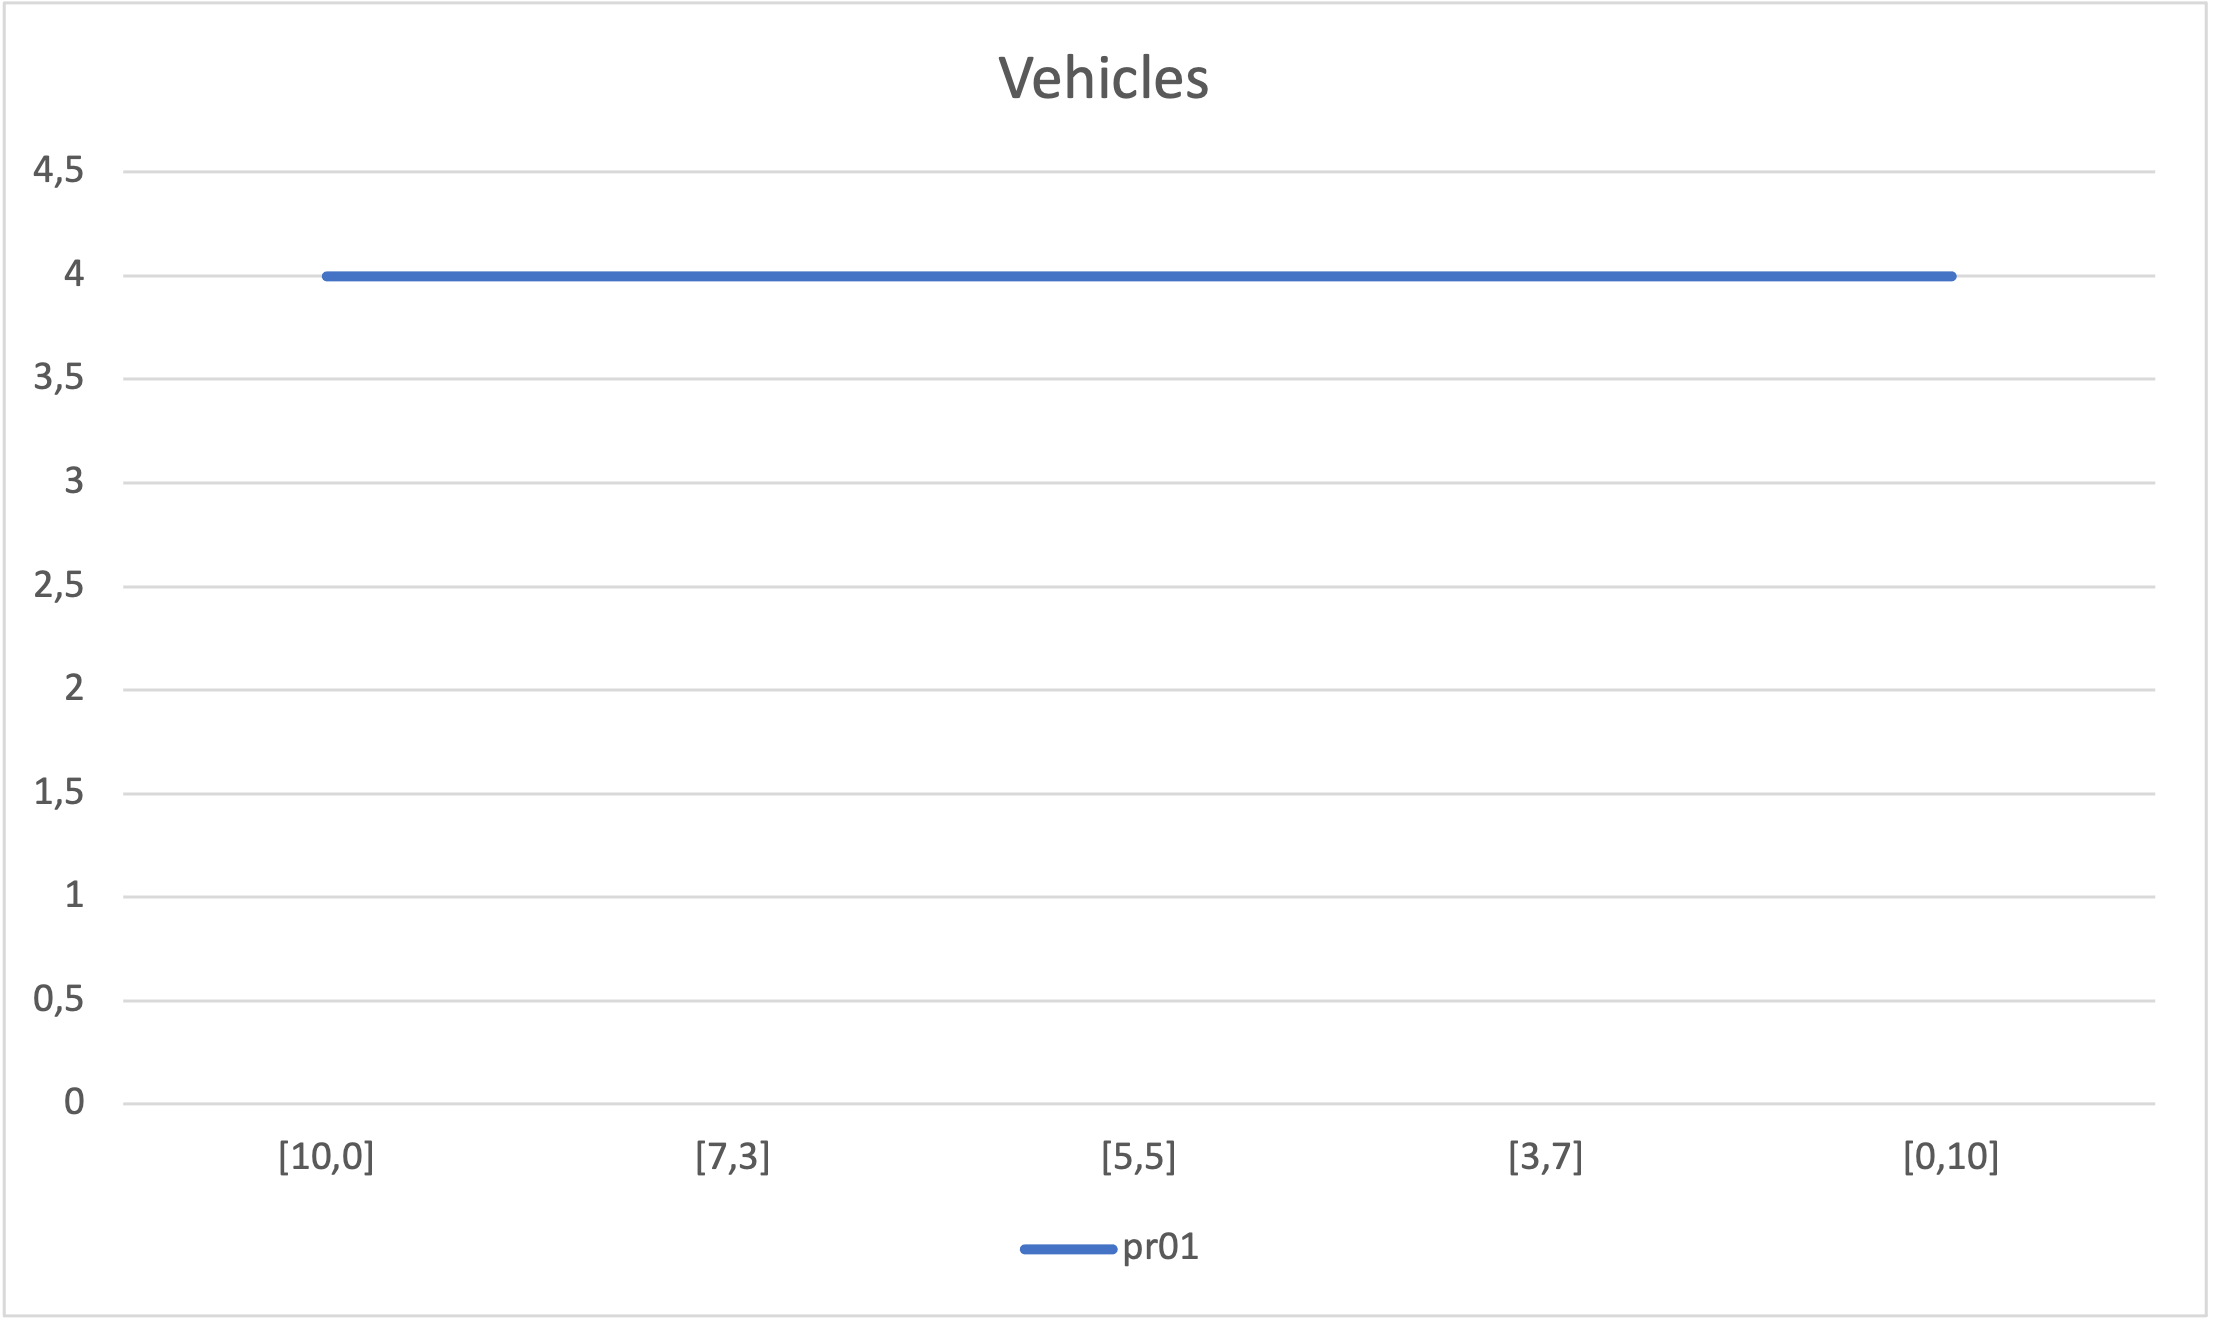
\includegraphics[height=0.25\textheight]{../graphs/pr01-vehicles.png}
    \caption{Vehicles used graph for \textbf{pr01}.}
\end{figure}

\newpage
